% ==========================================
% BAB II STUDI LITERATUR
% ==========================================
\chapter{STUDI LITERATUR}
\label{chap:studi-literatur}

% Anda dapat menambahkan pengantar umum untuk bab ini di sini jika diperlukan.
% \lipsum[1] % Contoh teks pengisi

\section{Pembelajaran Adaptif dan Asesmen Adaptif}
\label{sec:adaptive_learning_assessment}
Lingkungan pembelajaran adaptif (\textit{adaptive learning environments}) bertujuan
untuk meningkatkan perolehan pembelajaran individu dan pengalaman siswa dalam
lingkungan pembelajaran yang dipersonalisasi. Untuk mendukung pengembangan lingkungan
pembelajaran adaptif secara efektif, diperlukan metode asesmen pengetahuan yang
efisien untuk menilai keterampilan siswa secara empiris \autocite{Minn2022}. Penilaian
pembelajar adalah salah satu momen utama dalam proses pendidikan.

% \subsection{Definisi dan Prinsip Pembelajaran Adaptif}
Pembelajaran adaptif (\textit{adaptive learning}), secara definisi, adalah metodologi
untuk menyesuaikan dan mempersonalisasi proses pembelajaran, terutama konten, kepada
seorang pembelajar, agar sesuai dengan situasi dan keadaan yang berbeda. Tujuan dari
\textit{adaptive learning system} (ALS) atau sistem pembelajaran adaptif
adalah untuk mengubah instruksi menggunakan seperangkat aturan yang telah
ditentukan untuk menyediakan materi pembelajaran yang disesuaikan dengan
kebutuhan dan perilaku siswa. Pembelajaran adaptif memberikan kemungkinan
untuk menjadikan pembelajar sebagai kolaborator dalam proses pendidikan
alih-alih penerima informasi pasif, karena setiap pembelajar memiliki jalur
pembelajaran optimal spesifik yang terdiri dari banyak titik terhubung, dan setiap
titik mewakili komponen pengetahuan atau keterampilan \autocite{Ihichr2024}.

Pembelajaran adaptif mempertimbangkan banyak aspek, seperti tingkat pembelajar saat
ini, kebutuhan individu, gaya belajar, dan interaksi yang berbeda dengan siswa untuk
mengindividualisasi semua komponen proses pembelajaran: konten, antarmuka, gaya
belajar, dan asesmen. Oleh karena itu, pembelajaran adaptif memungkinkan seorang
siswa untuk maju ke materi yang lebih menantang berdasarkan kinerjanya, sambil di
sisi lain tetap memberikan dukungan tambahan kepada siswa lainnya untuk menguasai
keterampilan tertentu. Pendekatan ini memastikan bahwa pembelajar tidak dibatasi
oleh kecepatan kelas tetapi dapat mengikuti kecepatan belajar mereka sendiri.
Dengan demikian, instruktur dan pembelajar dapat membuat keputusan yang tepat
pada saat yang tepat dengan mengikuti kurva belajar dan lintasan belajar
(\textit{learning path}). Singkatnya, pembelajaran adaptif berusaha untuk menyesuaikan
pengalaman pendidikan untuk membantu siswa mencapai tujuan pembelajaran mereka
dengan meniru interaksi personalisasi satu lawan satu antara seorang guru dan
seorang pembelajar \autocite{Ihichr2024}.

% \subsection{Peran Asesmen Adaptif}
Pernyataan oleh psikolog Lauren Resnick, "Apa yang kita nilai adalah apa yang kita
hargai. Kita mendapatkan apa yang kita nilai, dan jika kita tidak menilainya, kita 
tidak mendapatkannya", menunjukkan pentingnya asesmen sebagai langkah utama dan
kritis dalam proses pendidikan. Banyak sistem pembelajaran adaptif lebih fokus
pada asesmen daripada konten. Data asesmen yang dikumpulkan dari respons siswa
digunakan untuk mempersonalisasi proses pembelajaran, menciptakan jalur yang
disesuaikan berdasarkan hasil. Jalur ini terus diperbarui dengan setiap asesmen.
Dengan demikian, asesmen pembelajar dianggap sebagai faktor krusial untuk proses
\textit{e-learning} yang sukses \autocite{Ihichr2024}.

Berbeda dengan pengujian konvensional, yang didasarkan pada \textit{item} tetap yang
harus dihadapi setiap peserta ujian terlepas dari tingkat pengetahuan mereka,
asesmen adaptif memungkinkan pemilihan pertanyaan berdasarkan kinerja peserta
ujian. Sistem asesmen adaptif secara terus-menerus menyesuaikan kembali proses
asesmennya sehubungan dengan tingkat kesulitan, dan sesuai dengan kinerja,
preferensi, motivasi, pengetahuan, serta tujuan pendidikan yang diekspresikan
oleh pembelajar \autocite{Halkiopoulos2024}. Asesmen adaptif menyediakan tes
singkat yang dipersonalisasi, \textit{item}-nya berubah tergantung pada respons
siswa, dan kesulitan setiap pertanyaan berkorelasi dengan jawaban pertanyaan
sebelumnya. Singkatnya, asesmen adaptif berusaha menghindari penyajian pertanyaan
mudah kepada siswa yang mampu, yang kemungkinan akan menjawab dengan benar, dan
pertanyaan menantang tidak disajikan kepada siswa yang kesulitan \autocite{Ihichr2024}.

\subsection{Jenis Penilaian}
Menurut \textcite{Ihichr2024}, asesmen pengetahuan secara global dapat dibagi menjadi
tiga jenis: sumatif, formatif, dan pra-asesmen. Umumnya, asesmen sumatif lebih
dominan daripada asesmen formatif dalam \textit{e-learning}, tetapi dua jenis
terakhir telah menunjukkan potensi lebih, terutama dalam pembelajaran adaptif.


\begin{enumerate}
    % \subsubsection{Asesmen Sumatif}
    \item Asesmen sumatif juga dikenal sebagai asesmen pembelajaran (\textit{assessment of
    learning}), jenis evaluasi ini terjadi di akhir siklus pembelajaran untuk mengukur
    pencapaian pembelajar dan memverifikasi penguasaan unit kurikulum. Asesmen ini
    bertujuan menilai kemajuan kumulatif pembelajar \autocite{Ihichr2024}. Informasi
    dari asesmen sumatif dapat digunakan secara formatif untuk memandu aktivitas
    mereka di pembelajaran selanjutnya \autocite{Minn2022}.

    % \subsubsection{Asesmen Formatif}
    \item Asesmen formatif atau yang disebut juga asesmen untuk pembelajaran
    (\textit{assessment for learning}), ini terjadi sepanjang siklus pembelajaran
    untuk memberikan informasi umpan balik kepada tutor dan pembelajar untuk membantu
    meningkatkan pengalaman belajar mereka. Jenis asesmen ini menilai kualitas
    pembelajaran dengan memposisikan asesmen antara pengajaran dan pembelajaran
    (kemajuan saat ini) alih-alih diposisikan hanya di akhir proses. Ketika asesmen
    formatif begitu tertanam dalam lingkungan pembelajaran sehingga pemisahan antara
    asesmen dan pembelajaran benar-benar kabur dan tidak terlihat oleh siswa, konsep
    ini dikenal sebagai \textit{stealth assessment}. Asesmen formatif memungkinkan kita
    untuk menyempurnakan lintasan pembelajaran, meningkatkan keterlibatan dan antusiasme
    siswa untuk menguasai suatu materi pembelajaran dan mengembangkan disiplin dalam
    dirinya \autocite{Ihichr2024}.
    
    % \subsubsection{Pra-Asesmen}
    \item Pra-asesmen atau yang dikenal sebagai asesmen diagnostik, jenis asesmen ini
    mengukur kompetensi awal setiap pembelajar, memberikan gambaran yang jelas kepada
    guru tentang tingkat keterampilan pembelajar. Ini seringkali diikuti oleh semacam
    instruksi kompensasi untuk menghilangkan hambatan dan menawarkan berbagai jenis
    kegiatan remedial. Pra-asesmen biasanya dilakukan di awal pembelajaran dan dirancang
    untuk mengukur pengetahuan yang sudah diperoleh sebelumnya oleh siswa untuk
    mengidentifikasi kebutuhan, kompetensi, prasangka, dan pengetahuan sebelumnya
    dari siswa tersebut, untuk mengarahkan mereka ke kurikulum yang paling sesuai
    \autocite{Ihichr2024}.
\end{enumerate}

\subsection{Luaran yang Dinilai}
\textcite{Ihichr2024} mendefinisikan tiga hasil pembelajaran utama yang dinilai
dalam pembelajaran daring, yaitu hasil pembelajaran kognitif, perilaku, dan afektif.
Studi tersebut menunjukkan bahwa ketiga aspek ini saling berkorelasi.

\begin{enumerate}
    % \subsubsection{Luaran Kognitif}
    \item \textbf{Luaran Kognitif:} luaran ini secara mendasar berkaitan dengan pengetahuan yang diperoleh dan
    keterampilan intelektual. Pengetahuan adalah semua informasi yang telah dipelajari
    siswa dari suatu topik, tetapi keterampilan intelektual menyangkut kemampuan yang
    berbeda, seperti penalaran, proses berpikir, dan pengambilan keputusan
    \autocite{Ihichr2024}.

    % \subsubsection{Luaran Perilaku}
    \item \textbf{Luaran Perilaku}: luaran perilaku merujuk pada pengukuran keterlibatan pembelajar dengan memantau
    perilakunya selama pembelajaran seperti durasi dan waktu belajar, partisipasi dalam
    forum dan diskusi, pengumpulan tugas, dan penyelesaian tes \autocite{Ihichr2024}.

    % \subsubsection{Luaran Afektif}
    \item \textbf{Luaran Afektif:} luaran ketiga ini berkaitan dengan persepsi siswa, kepuasan mereka terhadap pembelajaran,
    apresiasi terhadap pengalaman belajar mereka, dan manfaat yang diharapkan oleh mereka
    ketika mendaftarkan diri mengikuti suatu pembelajaran. Sebagian besar pembelajaran dan
    asesmen di pendidikan tinggi berkonsentrasi pada hasil kognitif daripada hasil afektif
    dan perilaku \autocite{Ihichr2024}.
\end{enumerate}

\subsection{Taksonomi Bloom dalam Asesmen Kognitif}

Kerangka kerja fundamental yang digunakan untuk mengklasifikasikan tujuan pendidikan dan mengukur kedalaman kognitif siswa adalah \textit{Bloom's Revised Taxonomy}. Sebagaimana dijelaskan oleh \textcite{Gosselin2018}, taksonomi ini membagi domain kognitif menjadi enam tingkatan hierarkis, yang bergerak dari proses berpikir tingkat rendah (\textit{lower-order cognition}) menuju tingkat tinggi (\textit{high-level cognition}). Tingkatan tersebut dimulai dari \textit{Remembering} (mengingat) dan \textit{Understanding} (memahami) sebagai fondasi dasar, kemudian berlanjut ke \textit{Applying} (menerapkan), \textit{Analyzing} (menganalisis), \textit{Evaluating} (mengevaluasi), hingga puncaknya pada \textit{Creating} (mencipta). Dalam konteks asesmen, idealnya \textit{Performance Indicators} (PI) dirancang dengan memadukan berbagai level ini sehingga siswa tidak hanya dituntut untuk mengingat fakta, tetapi juga menerapkan materi yang dipelajari dalam cara-cara yang kompleks. Penggunaan taksonomi ini memungkinkan penerjemahan luaran pembelajaran yang abstrak menjadi perilaku yang dapat diamati (\textit{observable behaviors}) dan diukur secara konkret.

Penerapan taksonomi ini dalam sistem asesmen memerlukan instrumen yang presisi, seperti penggunaan \textit{descriptive rubrics} (rubrik deskriptif). \textcite{Gosselin2018} menekankan bahwa penggunaan rubrik deskriptif yang diselaraskan dengan kata kerja operasional Bloom dapat meningkatkan konsistensi penilaian antarevaluator dan memberikan umpan balik yang lebih bermakna dibandingkan sekadar skala numerik generik. Rubrik ini mendeskripsikan variasi tingkat kinerja untuk setiap kriteria secara spesifik. Misalnya, dalam menilai kemampuan desain teknik, indikator kinerja direvisi dari sekadar berbasis topik menjadi berbasis level kognitif, seperti bergerak dari kemampuan "mengidentifikasi prinsip sains" (\textit{Understanding}) menuju kemampuan "membuat asumsi penyederhanaan dan mengevaluasi solusi" (\textit{Evaluating}). Pendekatan ini sangat relevan untuk asesmen sejawat (\textit{peer assessment}) karena rubrik yang terstruktur digunakan dalam asesmen untuk membantu siswa menilai kontribusi rekannya secara objektif berdasarkan deskripsi kinerja yang jelas, bukan sekadar persepsi subjektif.

Dalam disiplin ilmu komputasi, penggunaan kata kerja standar Bloom sering kali tidak memadai untuk menangkap nuansa teknis dari tugas-tugas pemrograman dan sistem informasi. Untuk mengatasi keterbatasan ini, \textcite{ACM2023} melalui \textit{ACM Committee for Computing Education in Community Colleges} (CCECC) mengusulkan peningkatan taksonomi dengan menambahkan 56 kata kerja spesifik komputasi (\textit{enhanced verbs}). Modifikasi ini memetakan aktivitas teknis ke dalam level kognitif yang sesuai. Sebagai contoh, aktivitas \textit{Code} (mengodekan), \textit{Build} (membangun), dan \textit{Decrypt} (mendekripsi) dikategorikan ke dalam level \textit{Applying}. Sementara itu, aktivitas yang membutuhkan pemecahan masalah lebih dalam seperti \textit{Debug} (men-debug), \textit{Optimize} (mengoptimalkan), dan \textit{Refactor} diposisikan pada level \textit{Evaluating}. Aktivitas sintesis seperti \textit{Script} (membuat skrip), \textit{Virtualize} (memvirtualisasi), dan \textit{Program} (membuat program solusi) ditempatkan pada level tertinggi, yaitu \textit{Creating}.

Integrasi kata kerja komputasi ini memungkinkan perancangan \textit{competencies} yang lebih akurat, yang didefinisikan sebagai integrasi antara pengetahuan (\textit{knowledge}), keterampilan (\textit{skills}), dan disposisi (\textit{dispositions}) dalam konteks tertentu \autocite{ACM2023}. Dalam lingkungan pembelajaran adaptif, pemetaan ini krusial untuk melacak progresi siswa. Seorang siswa mungkin memulai pembelajaran pada level \textit{Applying} dengan menerjemahkan spesifikasi menjadi kode, namun seiring waktu diharapkan berkembang ke level \textit{Creating} dengan mengimplementasikan solusi untuk masalah abstrak. \textcite{ACM2023} juga menyoroti bahwa disposisi atau aspek "sikap" (seperti \textit{collaborative} dan \textit{meticulous}) dapat dikaitkan dengan kompetensi teknis tersebut. Dengan demikian, sistem asesmen tidak hanya melacak kebenaran sintaksis kode, tetapi juga kedalaman pemahaman konseptual dan kemampuan kolaboratif siswa berdasarkan hierarki kognitif yang terstandarisasi.

% =====================================================================
% MULAI SUBBAB II.2 (BARU) - SISIPKAN SETELAH AKHIR SUBBAB II.1
% =====================================================================

\section{Pemodelan Siswa (\textit{Student Modeling})}
\label{sec:student_modeling}

Dalam konteks lingkungan pembelajaran adaptif, asesmen pengetahuan diperlukan
untuk membangun sebuah \textbf{\textit{student model}} (model siswa). Model
siswa adalah inti dari setiap sistem pendidikan adaptif, yang juga dikenal
sebagai \textit{learner model} \autocite{Brusilovsky2016}. Model ini berfungsi
sebagai blok pembangunan fundamental (\textit{fundamental building block}) dari
asesmen pengetahuan \autocite{Minn2022}. Tujuan utamanya adalah untuk
merepresentasikan keadaan pengetahuan domain (\textit{domain knowledge})
siswa saat ini. Selain pengetahuan, \textit{student model} juga dapat
merepresentasikan informasi lain tentang siswa seperti tujuan pembelajaran
(\textit{learning goals}), sifat-sifat personal (\textit{personal traits}),
dan/atau preferensi. Dengan menggunakan
\textit{student model} inilah sebuah sistem adaptif dapat menyediakan berbagai
intervensi pembelajaran yang dipersonalisasi, seperti
\textit{mastery learning} atau \textit{adaptive sequencing}
(pengurutan adaptif) \autocite{Brusilovsky2016}.

Untuk membangun \textit{student model} secara efektif, diperlukan sebuah
\textit{domain model} (model domain) sebagai landasan \autocite{Minn2022}.
\textit{Domain model} ini berfungsi untuk mengekstrak apa yang disebut sebagai
\textit{\textbf{Knowledge Components}} (KCs) atau keterampilan (\textit{skills})
dan atribut laten (\textit{latent attributes}) yang mendasari setiap tugas atau
materi pembelajaran. \textit{Knowledge Components} ini adalah
faktor laten (\textit{latents factors}) yang tidak pernah dapat diamati secara
langsung, namun keberadaannya dianggap menentukan hasil atau kinerja siswa pada
suatu tugas. Dalam kerangka kerja psikometri,
pemetaan antara \textit{item} (pertanyaan) dan KCs yang diperlukannya seringkali
direpresentasikan dalam sebuah \textit{\textbf{Q-matrix}} \autocite{Minn2022}.
Oleh karena itu, berbagai teknik asesmen adaptif (yang akan dibahas berikutnya)
pada dasarnya adalah algoritma yang digunakan untuk memperkirakan penguasaan
siswa atas KCs yang tersembunyi ini.

Dalam sebagian besar sistem pembelajaran terpersonalisasi,
\textit{student model} bersifat tersembunyi atau tidak dapat diamati
(\textit{unobservable}) oleh siswa, dan hanya digunakan oleh sistem untuk
menggerakkan adaptasi. Namun, sebuah pendekatan yang
dikenal sebagai \textbf{\textit{Open Student Modeling}} (OSM) atau
Pemodelan Siswa Terbuka, berusaha membuat terobosan baru dengan secara sengaja
memperlihatkan aspek-aspek model tersebut kepada pembelajar. Tujuan dari
pendekatan OSM adalah untuk meningkatkan \textit{self-reflection} (refleksi diri)
siswa, \textit{self-regulated learning} (pembelajaran mandiri),
transparansi personalisasi, dan motivasi siswa
\autocite{Brusilovsky2016, Ihichr2024}.

Sebuah ekstensi yang lebih baru dan relevan dengan penelitian ini adalah
\textbf{\textit{Open Social Student Modeling}} (OSSM) atau
Pemodelan Siswa Sosial Terbuka. Ide dari OSSM adalah untuk
melengkapi aspek kognitif OSM dengan aspek sosial.
Hal ini dicapai dengan mengizinkan siswa untuk mengeksplorasi model-model
rekan siswa dan/atau model kelas yang diagregasi. Pendekatan ini memiliki
kesamaan dengan teknik \textit{gamification} seperti \textit{leaderboards}
(papan peringkat), yang bertujuan memanfaatkan perbandingan sosial untuk
meningkatkan motivasi dan keterlibatan siswa. Penelitian telah menunjukkan
bahwa antarmuka OSSM, seperti yang diimplementasikan dalam \textit{MasteryGrids},
dapat "meningkatkan pembelajaran, terutama untuk siswa dengan pengetahuan awal
yang lebih rendah" \autocite{Brusilovsky2016}.

% =====================================================================
% AKHIR SUBBAB II.2 (BARU)
% =====================================================================

\section{Teknik dan Algoritma \textit{Adaptive Assessment}}
\label{sec:teknik_algoritma_aa}
Dalam rangka mencapai adaptivitas, sistem pembelajaran perlu memperkirakan tingkat 
kompetensi siswa dan tingkat kesulitan konten pendidikan \autocite{Vesin2022}. 
Berbagai teknik dan algoritma telah dikembangkan untuk memungkinkan asesmen adaptif, 
masing-masing dengan dasar teoretis dan karakteristiknya sendiri. Bagian ini mengulas
beberapa pendekatan utama yang digunakan dalam asesmen adaptif, dengan fokus pada 
\textit{Item Response Theory} (IRT), IRT* atau \textit{Bayesian IRT}, \textit{Hidden Markov Models} (HMM),
\textit{Factor Analysis} (FA), \textit{Bayesian Knowledge Tracing} (BKT),
\textit{Deep Knowledge Tracing} (DKT), dan sistem \textit{Elo rating}.

\subsection{\textit{Item Response Theory} (IRT)}
\textit{Item Response Theory (IRT)} adalah salah satu teori yang paling banyak
digunakan dalam asesmen adaptif, dengan asal-usulnya berasal dari Rasch dan Lord 
pada tahun 1950-an. Teori psikometri ini digunakan untuk memperkirakan pengetahuan 
pembelajar, mengembangkan pengukuran kognitif atau non-kognitif pembelajar, memilih 
pertanyaan berikutnya yang sesuai pada setiap momen, dan memutuskan kapan tes selesai 
\autocite{Ihichr2024}. Dalam IRT, probabilitas keberhasilan pada suatu tugas 
(\textit{item}) dipetakan sebagai fungsi dari tingkat kemahiran (\textit{ability}) 
yang mempertimbangkan keseluruhan tugas, dengan asumsi bahwa keadaan pengetahuan 
siswa statis selama ujian. Keadaan pengetahuan siswa $\theta$ dinilai berdasarkan
kemahirannya saat tes dilakukan, dan setiap \textit{item} yang diuji membantu
memberikan informasi untuk menyempurnakan estimasi keadaan pengetahuan $\theta_{i}$. 
Model IRT dasar mengasumsikan satu keterampilan tunggal dan bahwa \textit{item} 
tes bersifat unidimensional \autocite{Minn2022}. Secara formal, model IRT dasar
bisa diekspresikan dengan rumus matematika seperti berikut ini.

\begin{align}
P_{ij} &= \sigma(\theta_i - \beta_j) \notag \\
     &= \frac{1}{1 + e^{\theta_i - \beta_j}} \label{eq:rumus_irt}
\end{align}

Model IRT bisa dirancang dengan berbagai variasi parameter logistik.
Model IRT dengan 1-Parameter Logistik 
(1PL) hanya melibatkan satu karakteristik \textit{item}, yaitu kesulitan 
\textit{item} (b), sedangkan model 2PL melibatkan kesulitan \textit{item} (b) 
dan diskriminasi \textit{item} (a), dan model 3PL menambahkan karakteristik 
ketiga, yaitu tebakan (\textit{lower asymptote}) \textit{item} (c) 
\autocite{Handayani2025}. IRT bukanlah pendekatan \textit{Knowledge Tracing} 
karena mengasumsikan siswa tidak belajar selama proses pengujian; ini dianggap 
sebagai pendekatan \textit{Knowledge Assessment} \autocite{Minn2022}. Namun, IRT 
memiliki tantangan dalam hal kalibrasi pada sampel besar dan kesulitan komputasi 
untuk pembaruan yang sering karena estimasi keterampilan baru harus dihitung untuk 
setiap siswa setelah satu respons untuk satu tugas \autocite{Vesin2022}.

% \subsection{Model IRT* (\textit{Bayesian IRT})}
Selain pendekatan standar, model IRT juga dapat diterapkan dalam
kerangka kerja Bayesian (\textit{Bayesian framework}), pendekatan ini
dalam \textcite{Minn2022} disebut sebagai IRT*. Pendekatan Bayesian untuk IRT
memungkinkan peneliti untuk memasukkan informasi sebelumnya
(\textit{prior information}) tentang parameter model. \textit{Prior} ini
dapat ditentukan dengan berbagai cara, seperti menggunakan estimasi parameter
dari studi sebelumnya atau menggunakan \textit{prior} yang tidak informatif
jika tidak ada informasi yang tersedia. Sebagai
contoh, dalam kerangka kerja ini, tingkat kesulitan sebuah \textit{item}
dapat diperkirakan dari \textit{item} lain yang serupa, atau kemampuan
siswa dapat diperkirakan dari kinerjanya (\textit{performance}) pada tugas-tugas
lain. Pendekatan ini memanfaatkan pendekatan Bayesian dan
melakukan regularisasi terhadap $log P_ij$ dengan menerapkan distribusi
standard \textit{normal prior} independen ke setiap $\theta_i$ dan $\beta_j$.
Dengan demikian, model ini memaksimalkan probabilitas log posterior dari {$\theta_i$, $\beta_j$}
jika diketahui data respons {r: (i, j, r, t) $\in$ D}, dengan r adalah respons biner (nilainya antara 0 dan 1),
t adalah waktu ketika respons diberikan, dan D adalah kumpulan \textit{tuple} (i, j, r, t) yang menunjukkan
semua respons yang diberikan oleh siswa i pada \textit{item} j pada waktu t. Dalam penelitian oleh \textcite{Minn2022},
model IRT* dapat dirumuskan sebagai berikut.

\begin{multline}
\log P(\{\theta_i\}, \{\beta_j\}|D) = \sum_{(i,j,r,t) \in D} r\log \sigma(\theta_i - \beta_j) + (1-r) \\
\log(1 - \sigma(\theta_i - \beta_j)) - \frac{1}{2}\sum_i \theta_i^2 - \frac{1}{2}\sum_j \beta_j^2 + C \label{eq:rumus_irt_star}
\end{multline}

% \subsection{\textit{Hidden Markov Models} (HMM)}
% \textit{Hidden Markov Model} (HMM) adalah model statistik yang mengasumsikan
% bahwa sistem yang dimodelkan adalah proses Markov dengan keadaan yang tidak
% teramati (\textit{hidden states}). Dalam konteks asesmen
% pengetahuan, keadaan tersembunyi adalah penguasaan siswa terhadap suatu
% keterampilan. HMM memiliki dua asumsi utama. Asumsi pertama adalah bahwa
% keadaan pada waktu $t$ hanya bergantung pada keadaan pada waktu $t-1$.
% Asumsi kedua adalah bahwa observasi (misalnya, jawaban siswa) pada waktu $t$
% hanya bergantung pada keadaan pada waktu $t$. Dalam model
% ini, keadaan pengetahuan siswa dimodelkan sebagai variabel laten yang bertransisi
% antar keadaan (misalnya, dari "belum dipelajari" ke "dipelajari"), dan
% probabilitas transisi ini diperbarui berdasarkan urutan kinerja siswa
% yang teramati \autocite{Minn2022}.

\subsection{\textit{Factor Analysis} (FA)}
\textit{Factor Analysis} (FA) atau Analisis Faktor adalah teknik psikometri
yang menjelaskan korelasi antar variabel yang teramati
(\textit{observed variables}). Dalam konteks
asesmen adaptif, FA utamanya berfungsi untuk membangun model pembelajar,
khususnya komponen kognitif, dengan mengeksplorasi faktor-faktor yang
memengaruhi proses pembelajaran. Faktor-faktor ini mungkin termasuk
pengetahuan sebelumnya (\textit{prior knowledge}), kemampuan kognitif,
dan motivasi. FA membantu dalam menentukan \textit{item}
yang paling baik mengukur kemahiran pembelajar dan dalam menghasilkan umpan
balik adaptif \autocite{Ihichr2024}.

Model berbasis FA memperkirakan kemahiran siswa pada setiap
atribut (keterampilan) sebagai variabel laten kontinu.
Model FA dapat dibagi menjadi dua kategori: \textit{exploratory factor
analysis} (EFA) dan \textit{confirmatory factor analysis} (CFA). EFA
digunakan untuk mengidentifikasi struktur faktor yang mendasari
(\textit{underlying factor structure}) dan mengurangi jumlah total
\textit{item} tes. CFA, di sisi lain, digunakan untuk memverifikasi
apakah struktur faktor yang dihipotesiskan konsisten dengan data
respons siswa. Dalam CFA, peneliti perlu menentukan
terlebih dahulu jumlah faktor laten dan \textit{item} mana yang terkait
dengan faktor mana sebelum melakukan analisis \autocite{Minn2022}.

\subsection{\textit{Hidden Markov Models} (HMM) dan \textit{Bayesian Knowledge Tracing (BKT)}}
\textit{Hidden Markov Model} (HMM) adalah model statistik yang mengasumsikan
bahwa sistem yang dimodelkan adalah proses Markov dengan keadaan yang tidak
teramati (\textit{hidden states}). Dalam konteks asesmen
pengetahuan, keadaan tersembunyi adalah penguasaan siswa terhadap suatu
keterampilan. HMM memiliki dua asumsi utama. Asumsi pertama adalah bahwa
keadaan pada waktu $t$ hanya bergantung pada keadaan pada waktu $t-1$.
Asumsi kedua adalah bahwa observasi (misalnya, jawaban siswa) pada waktu $t$
hanya bergantung pada keadaan pada waktu $t$. Dalam model
ini, keadaan pengetahuan siswa dimodelkan sebagai variabel laten yang bertransisi
antar keadaan (misalnya, dari "belum dipelajari" ke "dipelajari"), dan
probabilitas transisi ini diperbarui berdasarkan urutan kinerja siswa
yang teramati \autocite{Minn2022}.

Salah satu penerapan HMM yang paling luas dalam asesmen adaptif adalah
\textit{Bayesian Knowledge Tracing (BKT)}, suatu  pendekatan yang didasarkan pada 
\textit{Bayesian Networks} (BNs). Pendekatan ini mencoba memodelkan keterampilan 
pembelajar dengan menghitung probabilitas penguasaan keterampilan berdasarkan 
seperangkat parameter: menebak (\textit{guessing}), terpeleset (\textit{slipping}), 
probabilitas bahwa keterampilan sudah dikuasai sebelumnya, dan probabilitas bahwa 
keterampilan akan dipelajari. BKT memperhitungkan urutan waktu untuk memperkirakan 
keterampilan baru dan mengasumsikan bahwa setiap keterampilan yang dipelajari tidak 
pernah dilupakan \autocite{Ihichr2024}.

BKT adalah pendekatan paling awal untuk 
memodelkan keadaan pengetahuan pembelajar yang berubah dan merupakan model pertama 
yang melonggarkan asumsi keadaan pengetahuan statis. Dalam BKT standar, satu 
keterampilan tunggal diuji per \textit{item} dan keadaan penguasaan keterampilan 
pembelajar disimpulkan pada setiap langkah waktu berdasarkan urutan hasil sebelumnya. 
BKT mengandalkan model Markov untuk menyimpulkan keadaan penguasaan, dari "belum 
dipelajari" menjadi "dipelajari". Berbagai ekstensi BKT telah diperkenalkan, seperti 
memperhitungkan pengetahuan sebelumnya siswa atau kesulitan \textit{item} 
\autocite{Minn2022}.

\begin{figure}[!ht]
    \centering
    \captionsetup{justification=centering}
        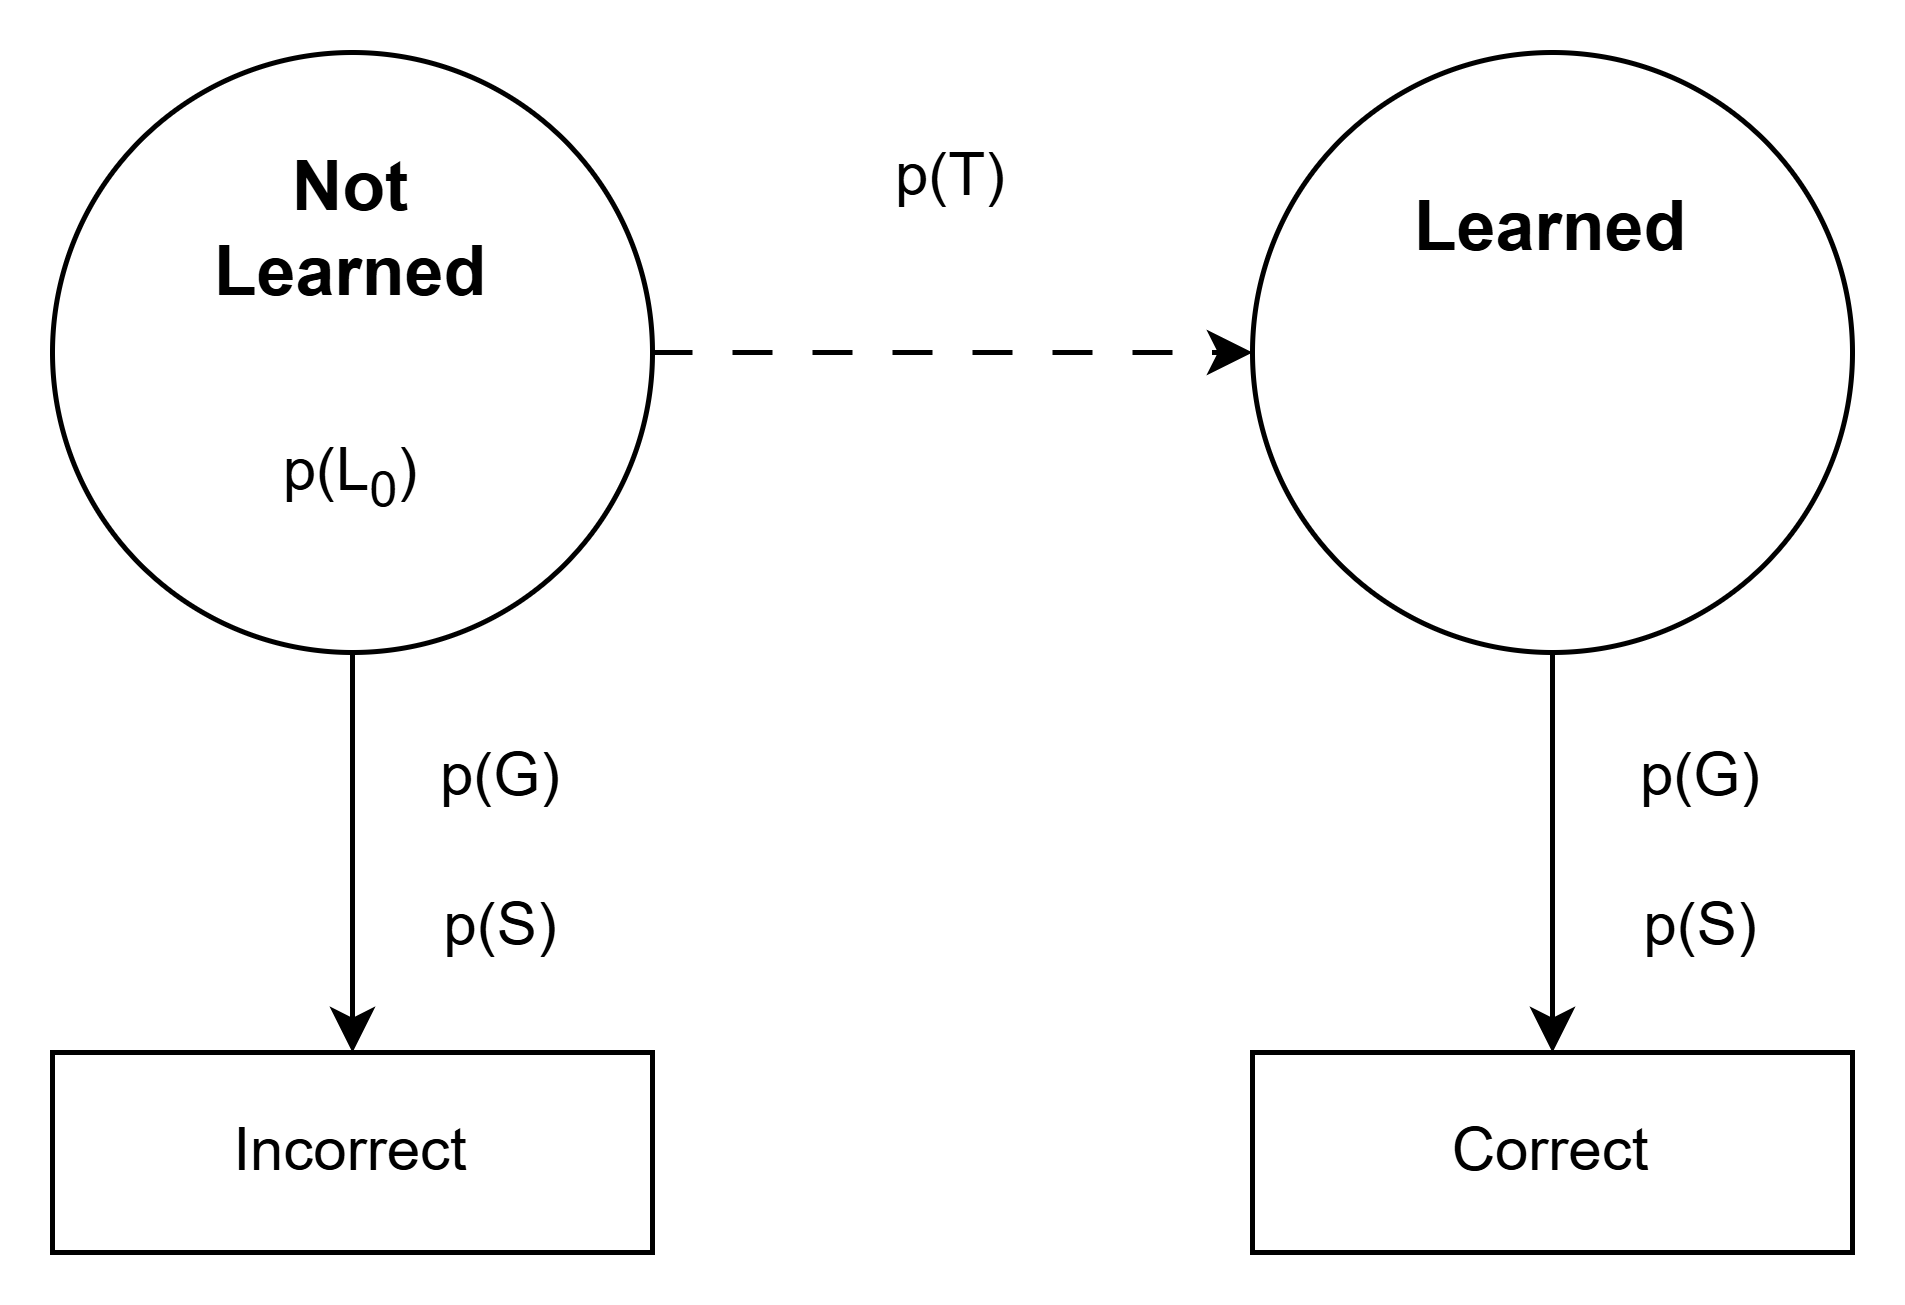
\includegraphics[width=0.9\textwidth]
        {image/standard_bkt.png}
    \caption{Contoh Model Konseptual dari BKT Standard yang Mengestimasi
    Transisi \textit{State} siswa dari Belum Dipelajari (\textit{Not Learned})
    menjadi Sudah Dipelajari (\textit{Learned}) (diadaptasi dari \textcite{Minn2022})}
    \label{fig:model-standard-bkt}
\end{figure}

\subsection{\textit{Deep Knowledge Tracing (DKT)}}
\textit{Deep Knowledge Tracing (DKT)}, sebuah algoritma perintis yang
menggunakan jaringan neural rekuren dalam (\textit{deep recurrent neural networks})
untuk memodelkan pembelajaran siswa dan melacak pengetahuan mereka, digunakan untuk
mengekstrak struktur laten antar asesmen. DKT bergantung pada model RNN dan LSTM,
yang menawarkan keuntungan signifikan dengan menangkap representasi pengetahuan yang
kompleks dari asesmen dari waktu ke waktu. Kemampuan ini memungkinkan kinerja 
prediksi yang jauh lebih baik di seluruh dataset dari asesmen sebelumnya. Selain itu,
model yang dipelajari dapat digunakan untuk merancang asesmen berikutnya yang lebih
sesuai untuk siswa \autocite{Ihichr2024}.

DKT menggunakan data yang diperoleh dari 
pengujian keterampilan dan hasil pengujiannya digunakan untuk memprediksi upaya 
urutan pembelajaran di masa mendatang. DKT menggunakan sejumlah besar neuron buatan 
untuk mewakili keadaan pengetahuan laten bersama dengan struktur dinamis temporal 
yang memungkinkan model untuk mempelajari keadaan pengetahuan siswa dari data. Namun,
seperti model \textit{deep learning} lainnya, DKT seringkali berfungsi sebagai 
\textit{black box} dengan sejumlah besar parameter dan struktur yang kompleks
sehingga sulit untuk memberikan penjelasan yang bermakna secara psikologis yang 
mencerminkan teori evolusi kognitif manusia \autocite{Minn2022}.

\subsection{Sistem \textit{Elo rating}}
Sistem \textit{Elo rating}, yang awalnya dikembangkan untuk memberi peringkat
pemain catur, baru-baru ini digunakan dalam pendidikan untuk mengatasi beberapa
celah yang ditimbulkan oleh model IRT. \textit{Elo rating} sepenuhnya bergantung
pada evaluasi kuantitatif kinerja siswa, dan dapat memodelkan keterampilan yang
berubah seiring waktu. Ketika \textit{item} baru ditambahkan dalam sistem, tidak
perlu menetapkan kesulitan \textit{item} awal yang benar, karena sistem akan belajar
dan menetapkan tingkat kesulitan untuk konten pendidikan, berdasarkan kebenaran
jawaban siswa. Terakhir, algoritma \textit{Elo rating} dapat memberikan estimasi
kesulitan tugas yang akurat dengan ukuran sampel kecil, sesuatu yang tidak mungkin
dilakukan dengan model IRT \autocite{Vesin2022}. Adaptasi \textit{Elo rating} ke
bidang pendidikan mengasumsikan bahwa siswa adalah pemain dan \textit{item} konten
(misalnya, latihan penulisan kode program) adalah lawan.

Peringkat \textit{Elo} siswa
dan konten diwakili oleh angka, yang meningkat atau menurun tergantung pada tindakan
siswa dengan sumber belajar. Perbedaan peringkat antara siswa dan \textit{item}
berfungsi sebagai prediktor hasil tindakan. Algoritma \textit{Elo rating} merupakan
algoritma yang hemat sumber daya komputasi, sangat sederhana untuk diimplementasikan,
dan cocok untuk praktik adaptif dalam pendidikan \autocite{Vesin2022}. Implementasi
yang diusulkan oleh \textcite{Vesin2022} memperluas \textit{Elo rating} klasik dengan
mempertimbangkan parameter tambahan seperti jumlah upaya dan waktu yang digunakan, 
bukan hanya status terselesaikan atau tidak, untuk memberikan adaptivitas dan
rekomendasi dalam tugas pemrograman \textit{open-ended}.

Secara spesifik, metode yang diusulkan menerapkan dua strategi, (1) memperbarui peringkat
berdasarkan performa siswa pada materi pembelajaran dibandingkan nilai ekspektasinya dan (2)
tingkat kesulitan konten pembelajaran diperbarui berdasarkan tingkat pemahaman siswa yang berhasil,
ataupun gagal dalam latihan. Secara matematis, cara ini mengestimasi probabilitas seorang siswa \textit{i} mampu
menyelesaikan latihan j berdasarkan peringkat siswa saat ini dan tingkat kesulitan latihan \textit{j}.
Peringkat siswa dan kesulitan latihan kemudian diperbarui menurut rumus berikut.

\begin{align}
R_i &= R_{i-1} + K (W - W_e)\label{eq:rumus_elo_student}
\end{align}
\begin{align}
D_j &= D_{j-1} + K (W_e - W)\label{eq:rumus_elo_latihan}
\end{align}

dengan $R_i$ adalah peringkat siswa setelah menyelesaikan latihan ke-i,
$R_{i-1}$ adalah peringkat siswa sebelum menyelesaikan latihan ke-i,
$D_j$ adalah tingkat kesulitan latihan ke-j setelah siswa menyelesaikannya,
$D_{j-1}$ adalah tingkat kesulitan latihan ke-j sebelum siswa menyelesaikannya,
$K$ adalah faktor penyesuaian yang menentukan seberapa besar perubahan peringkat
atau tingkat kesulitan, nilai ini dikurangi secara bertahap seiring siswa menyelesaikan lebih banyak latihan,
$W$ merepresentasikan hasil dari penyelesaian latihan yang direkomendasikan (dengan kata lain adalah tingkat keberhasilan),
yang dihitung berdasarkan formula berikut.

\begin{align}
W = \left(\frac{(A_s + A_o)T_c}{2A_oT_p}\right)(a_id_i - a_it_i). \label{eq:rumus_W_elo}
\end{align}

Rumus \ref{eq:rumus_W_elo} di atas adalah kunci modifikasi algoritma \textit{Elo rating} dari riset oleh \textcite{Vesin2022},
variabel-variabelnya dijelaskan dalam laporan hasil risetnya dengan definisi di bawah ini:
\begin{itemize}
    \item $A_s$: banyaknya upaya yang berhasil untuk latihan tertentu
    \item $A_o$: banyaknya total upaya untuk latihan tertentu
    \item $T_c$: banyaknya latihan yang sudah diselesaikan
    \item $T_p$: banyaknya latihan yang diselesaikan dengan benar
    \item $a_i$: bobot yang menentukan seberapa penting kecepatan (waktu) memengaruhi skor akhir
    \item $d_i$: merepresentasikan batas waktu
    \item $t_i$: merepresentasikan waktu yang dibutuhkan untuk menyelesaikan latihan
\end{itemize}

Terakhir adalah komponen $W_e$, komponen ini merepresentasikan probabilitas
seorang siswa mampu menyelesaikan latihan tertentu, yang dihitung berdasarkan rumus elo standard \autocite{Elo1978}:
\begin{align}
W_e = \frac{1}{1+10^{\frac{R_{i-1} - D_{j-1}}{400}}}. \label{eq:rumus_W_e_elo}
\end{align}

\subsection{Posisi Teknik dan Algoritma dalam Sistem Asesmen Adaptif Individual}
\label{ssec:arsitektur_sistem_aa_individual}
Berbagai teknik yang telah dibahas di atas (IRT, Elo rating, dll.) umumnya
diimplementasikan dalam sebuah siklus sistem.
Model konseptual siklus sistem yang dominan untuk asesmen adaptif
saat ini adalah siklus yang
berpusat pada pembelajar tunggal. Sebuah contoh representatif dari alur kerja ini
diimplementasikan dalam sistem ProTuS oleh \textcite{Vesin2022}, seperti yang
ditunjukkan pada Gambar \ref{fig:model-konseptual-individu}.

\begin{figure}[!ht]
    \centering
    \captionsetup{justification=centering}
        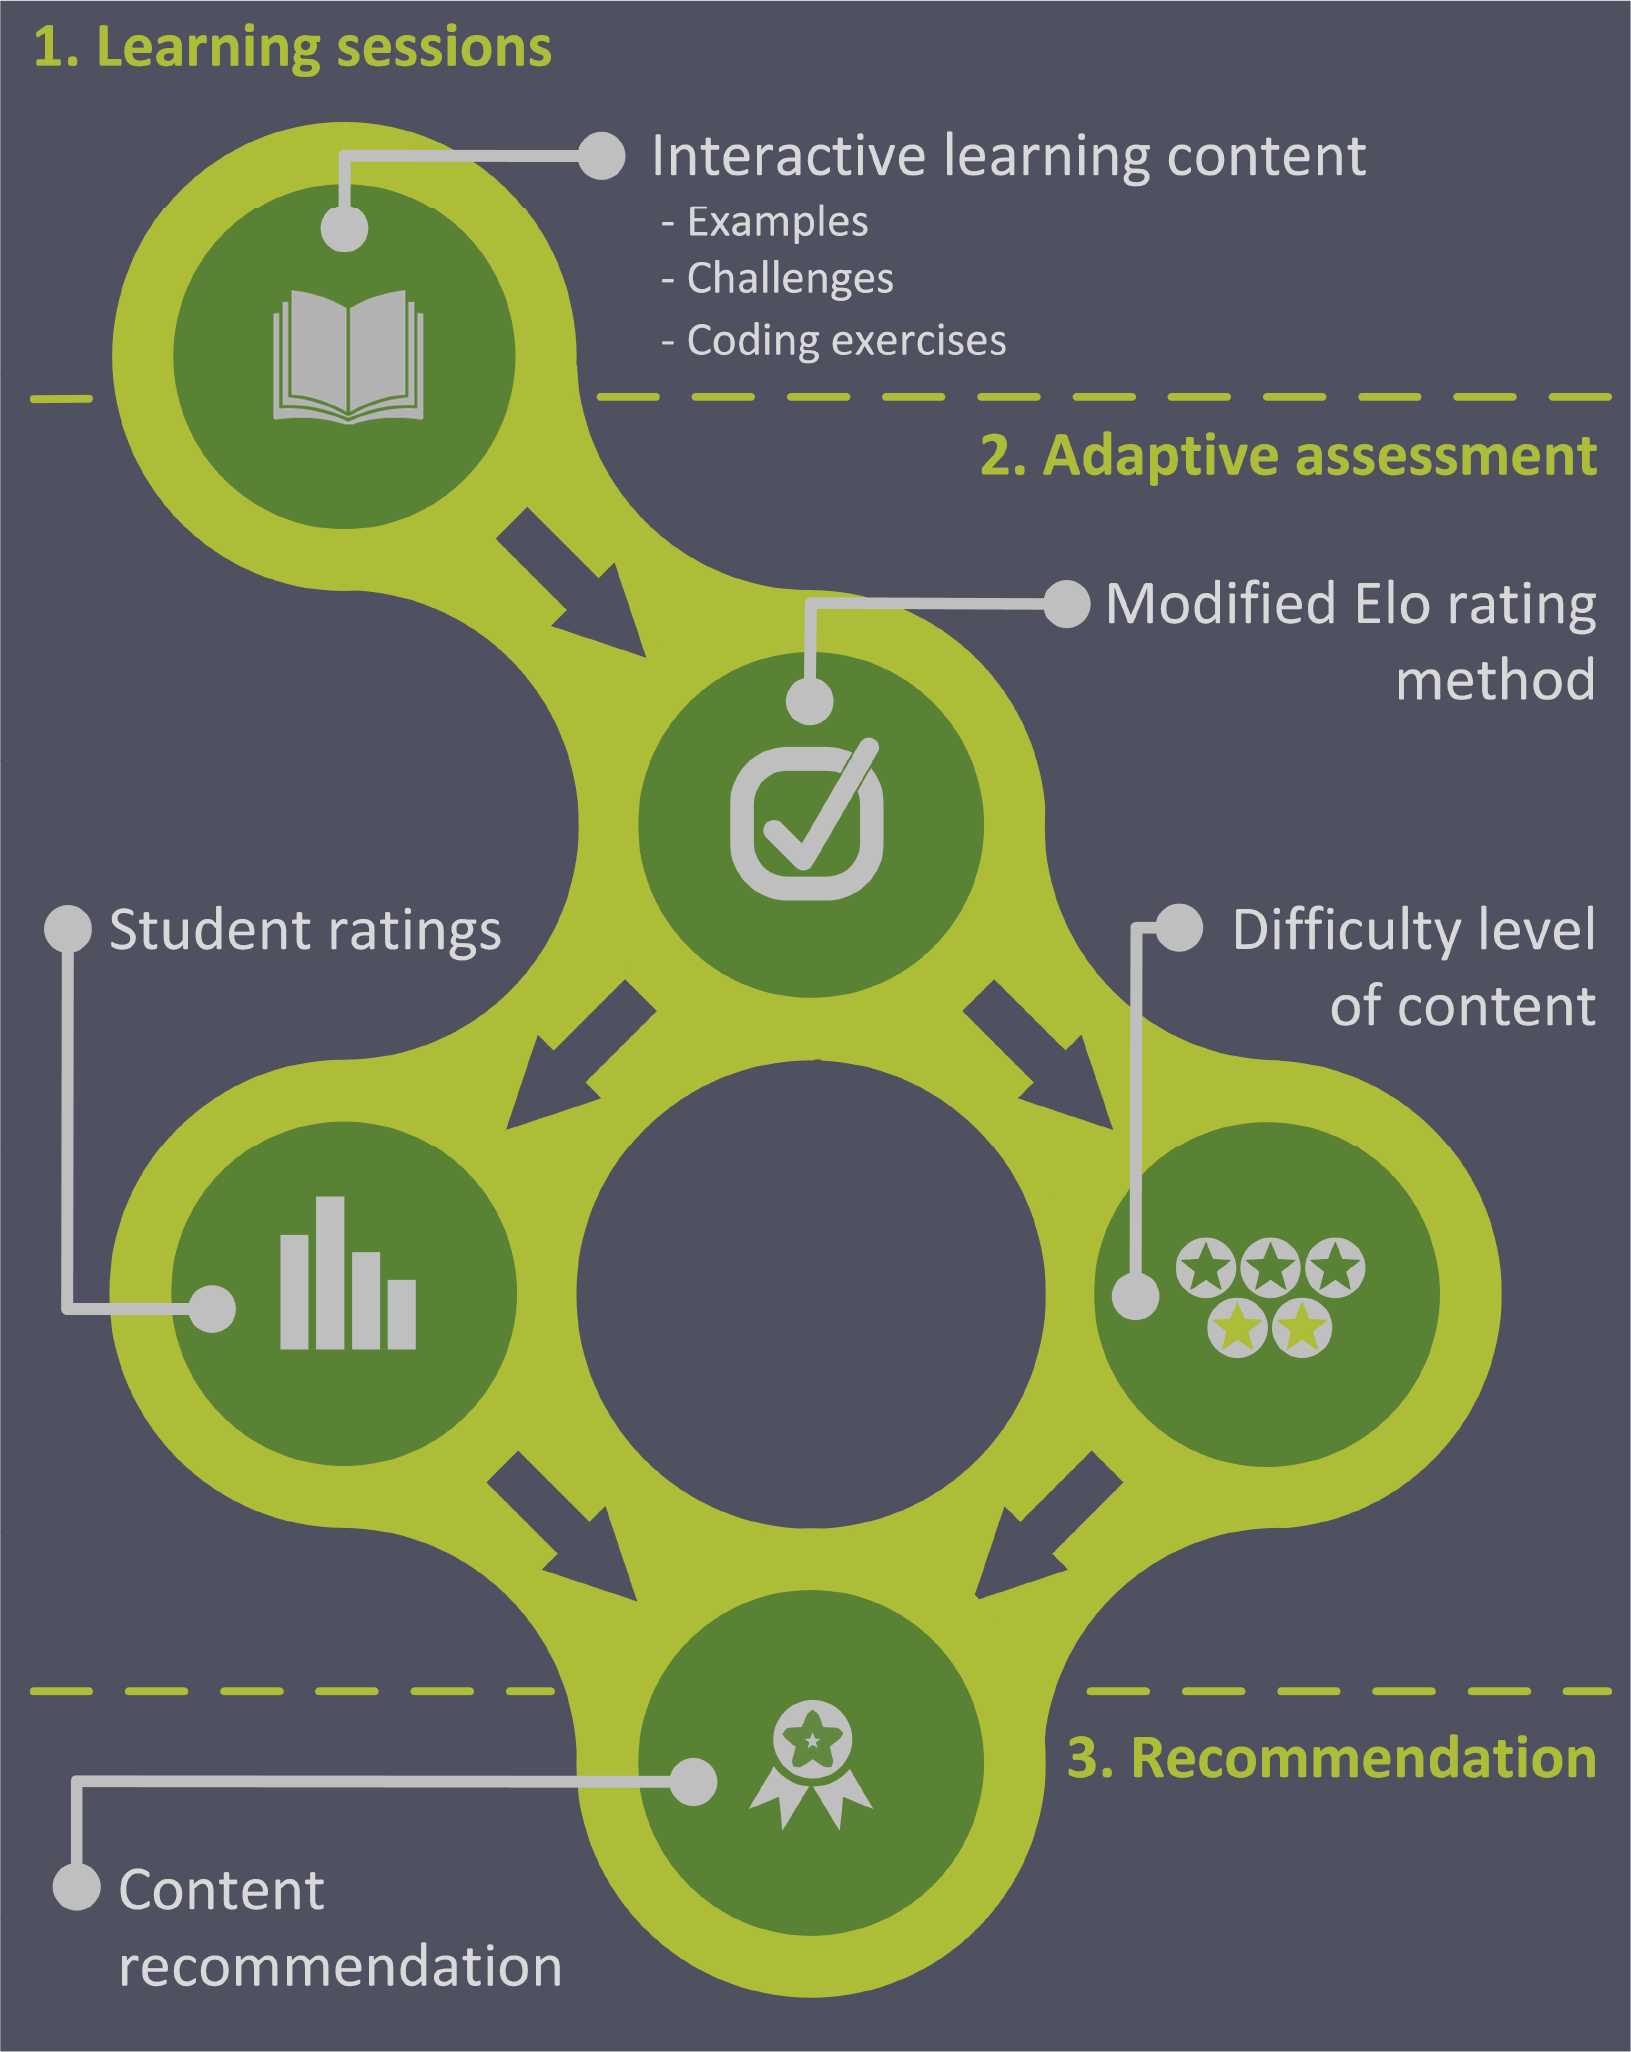
\includegraphics[width=0.8\textwidth]
        {image/vesin_fig1.png}
    \caption{Model Konseptual Alur Proses Sistem Adaptif
    Individual (diadaptasi dari \textcite{Vesin2022})}
    \label{fig:model-konseptual-individu}
\end{figure}

Menurut \textcite{Vesin2022} alur proses dalam model ini terdiri dari tiga tahap
yang diulang secara terus-menerus:
\begin{enumerate}
    \item \textbf{Sesi Pembelajaran (\textit{Learning Sessions}):} Siswa berinteraksi
    dengan sumber daya pembelajaran yang disediakan, seperti membaca materi
    atau menyelesaikan latihan pengkodean.
    \item \textbf{Asesmen Adaptif (\textit{Adaptive Assessment}):} Saat siswa
    menyelesaikan aktivitas, sistem memperbarui peringkat mereka berdasarkan
    kinerja individu. Peringkat siswa
    (\textit{student ratings}) dan tingkat kesulitan konten
    (\textit{difficulty level of content}) dihitung menggunakan metode seperti
    \textit{Elo rating} yang dimodifikasi.
    \item \textbf{Rekomendasi (\textit{Recommendation}):} Sistem kemudian 
    merekomendasikan aktivitas pembelajaran lebih lanjut yang sesuai dengan
    kemahiran siswa saat ini.
\end{enumerate}

Tahap modifikasi kesulitan konten pembelajaran mungkin tidak ada di semua sistem
karena beberapa teknik seperti IRT mengharuskan kesulitan konten ditetapkan sebelumnya.
Namun, secara umum akan melalui siklus seperti di atas, dan teknik serta algoritma
yang dibahas sebelumnya berperan secara khusus dalam tahap asesmen adaptif.

% Masalah pada model ini adalah bahwa keseluruhan siklus bersifat individualistis.
% Algoritma asesmen (misalnya, \textit{Elo rating} yang dimodifikasi) menghitung
% keberhasilan siswa murni berdasarkan parameter individual, seperti
% "jumlah upaya yang berhasil/gagal", "persentase/tingkat keberhasilan
% \textit{unit test}", dan "waktu yang dibutuhkan untuk menyelesaikan latihan"
% \autocite{Vesin2022}. Model ini tidak memiliki mekanisme untuk memasukkan
% atau mengukur nilai dari interaksi sosial.

\section{Pembelajaran Kolaboratif dan CSCL}
\label{sec:collaborative_learning}
Tantangan untuk beralih dari model pedagogi yang berpusat pada instruktur menjadi
berpusat pada siswa \autocite{Ryoo2021} sejalan dengan penekanan Strategi Nasional
KA Indonesia pada pentingnya ekosistem kolaboratif \autocite{BPPT2020}. Dalam konteks
pendidikan, filosofi kolaboratif ini sering dimediasi oleh teknologi melalui
\textit{Computer-Supported Collaborative Learning} (CSCL). Bagian ini membahas
prinsip-prinsip dan tantangan dari pendekatan sosial ini, yang menjadi landasan
untuk komponen "sosial" dari sistem yang diusulkan.

\subsection{Prinsip Pembelajaran Kolaboratif berbasis Teknologi}
\label{ssec:prinsip_cscl}
Alih-alih mendefinisikannya secara kaku, pendekatan modern melihat pembelajaran
kolaboratif sebagai proses yang memanfaatkan teknologi untuk mendukung interaksi
sosial. Prinsip-prinsip utamanya meliputi:

\begin{enumerate}
    \item \textbf{Konstruksi Pengetahuan Sosial:} Sistem pembelajaran dapat didasarkan
    pada pendekatan konstruktivis sosial. Dalam model ini, pembelajaran muncul melalui
    interaksi baik dengan rekan yang berpengetahuan (\textit{knowledgeable peers})
    atau dengan sistem AI. Tujuannya adalah untuk mendorong formasi kelompok yang
    heterogen untuk memaksimalkan keragaman kognitif dan mendorong refleksi kritis
    \autocite{Halkiopoulos2024}.

    \item \textbf{Interaksi dalam Komunitas Praktik \textit{(Communities of Practice)}:
    } Teknologi dapat memfasilitasi pembentukan \textit{Communities of Practice} (CoP).
    Sistem \textit{Computer-Supported Collaborative Work} (CSCW) atau proyek berbasis
    tim (\textit{team-based projects}) memungkinkan pembelajar untuk berinteraksi
    dalam ruang tiga dimensi yang sama meskipun secara fisik berada di lokasi yang
    jauh \autocite{Ryoo2021}.
\end{enumerate}

Meskipun prinsip pembentukan kelompok heterogen telah diakui kepentingannya,
tantangan teknis dalam sistem adaptif adalah menentukan standar kuantitatif yang
baku untuk menilai apakah perbedaan kemampuan antar-siswa sudah cukup signifikan
untuk disebut heterogen.

\subsection{Pengukuran Heterogenitas Kelompok dan \textit{Effect Size}}

Dalam ranah ilmu perilaku dan pendidikan, pengukuran perbedaan antara dua kelompok
atau individu tidak cukup hanya dengan melihat selisih nilai mentah (\textit{raw
score differences}), karena nilai tersebut sangat bergantung pada satuan skala
yang digunakan. Untuk mengatasi hal ini, \textcite{Cohen1988} memperkenalkan
konsep \textit{Effect Size} (ES) sebagai indeks standar yang independen dari
satuan pengukuran asal. Salah satu indeks ES yang paling fundamental dan banyak
digunakan untuk membandingkan dua rata-rata adalah \textit{Cohen's d}. Secara
konseptual, \textit{Cohen's d} didefinisikan sebagai selisih antara dua rata-rata
populasi ($m_A - m_B$) yang dibagi dengan standar deviasi populasi ($\sigma$).
Rasio ini merepresentasikan jarak antara dua rata-rata dalam satuan unit
variabilitas standar, memberikan ukuran murni mengenai seberapa jauh dua
distribusi nilai terpisah satu sama lain.

Dalam praktiknya, ketika parameter populasi tidak diketahui, nilai $d$ diestimasi
menggunakan statistik sampel. \textcite{Cohen1988} merumuskan penghitungan $d$
untuk dua sampel independen dengan menggunakan \textit{pooled standard deviation}
($\sigma_{pooled}$) sebagai penyebut, yang merupakan rata-rata akar kuadrat dari
varians kedua kelompok. Rumus formal untuk menghitung jarak atau indeks perbedaan
ini dinyatakan sebagai:

\begin{align}
    d &= \frac{| \bar{x}_A - \bar{x}_B |}{\sigma_{pooled}} \label{eq:cohen_d_basic} \\
    \sigma_{pooled} &= \sqrt{\frac{(n_A-1)s_A^2 + (n_B-1)s_B^2}{n_A + n_B - 2}} \label{eq:sigma_pooled}
\end{align}

dengan $\bar{x}_A$ dan $\bar{x}_B$ adalah nilai rata-rata (atau skor kemampuan
individu) dari dua entitas yang dibandingkan, $s_A^2$ dan $s_B^2$ adalah varians
masing-masing, serta $n_A$ dan $n_B$ adalah ukuran sampel. Jika diaplikasikan pada
perbandingan antar-individu (dengan $n=1$), penyebut dapat disederhanakan menjadi
standar deviasi gabungan dari populasi referensi atau data historis sistem. Nilai
$d$ yang dihasilkan adalah nilai skalar tak berdimensi yang memungkinkan
perbandingan yang adil lintas konteks yang berbeda.

Untuk memberikan makna interpretatif pada nilai numerik $d$, \textcite{Cohen1988} menetapkan standar konvensi yang telah menjadi rujukan universal dalam analisis kuantitatif. Konvensi ini dirancang untuk memetakan besaran statistik ke dalam dampak kualitatif yang dapat diamati di dunia nyata.
\begin{enumerate}
    \item \textbf{Efek Kecil ($d = 0.2$):} Perbedaan yang nyata namun sulit dideteksi tanpa analisis statistik yang cermat.
    \item \textbf{Efek Sedang ($d = 0.5$):} Perbedaan yang cukup besar untuk dapat dilihat oleh mata telanjang pengamat yang berpengalaman (\textit{visible to the naked eye}).
    \item \textbf{Efek Besar ($d = 0.8$):} Perbedaan yang sangat mencolok, setara dengan perbedaan tinggi badan antara remaja usia 13 dan 18 tahun.
\end{enumerate}
Standar operasional ini memberikan landasan teoretis yang kokoh untuk menetapkan ambang batas (\textit{threshold}) dalam menentukan apakah dua entitas (atau kelompok) dapat dikategorikan "berbeda secara signifikan" atau heterogen dalam konteks intervensi pendidikan.

\subsection{Aktivitas Pembelajaran Sosial dan Dampaknya}
\label{ssec:aktivitas_pembelajaran_sosial}
Selain prinsip-prinsip umum yang telah dibahas pada Subbab
\ref{ssec:prinsip_cscl}, penting untuk mengidentifikasi bentuk-bentuk aktivitas
pembelajaran sosial spesifik yang telah terbukti secara empiris memiliki dampak
positif terhadap hasil belajar. Aktivitas-aktivitas inilah yang menjadi kandidat
utama untuk diintegrasikan dan dinilai dalam sebuah sistem adaptif.

\begin{enumerate}
    % \subsubsection{Penilaian Sejawat (\textit{Peer Assessment})}
    % \label{sssec:peer_assessment}
    \item \textbf{Penilaian sejawat (\textit{Peer Assessment}):}
    Penilaian sejawat adalah aktivitas pendidikan yang mengajak
    siswa saling menilai pekerjaan rekannya, artinya dalam
    penilaian ini "penilai (\textit{assessor}) dan yang dinilai
    (\textit{assessed}) memiliki status yang sama"
    \autocite{Ihichr2024}.
    
    Evaluasi terhadap kinerja asesor dalam
    \textit{peer assessment} tidak cukup hanya didasarkan
    pada akurasi skor (\textit{rating accuracy}), tetapi
    juga harus meninjau kualitas umpan balik tekstual yang
    diberikan secara terukur. \textcite{Kerman2024}
    mengembangkan skema pengkodean yang membagi fitur umpan
    balik ke dalam tiga elemen utama: (1) \textit{Affective}
    (afektif), yang mencakup emosi positif seperti pujian
    atau emosi negatif; (2) \textit{Cognitive} (kognitif),
    yang terdiri dari deskripsi ringkasan (\textit{description}),
    identifikasi masalah (\textit{identification}), dan
    justifikasi masalah (\textit{justification}),
    serta (3) \textit{Constructive} (konstruktif)
    yang mencakup rekomendasi solusi.
    
    Keunggulan dari pendekatan ini adalah kemampuannya
    untuk mengkuantifikasi kualitas umpan balik secara
    granular. Dalam rubrik yang diusulkan
    \textcite{Kerman2024}, setiap fitur dinilai dengan
    skor dari nol (kualitas buruk) hingga dua (kualitas baik).
    Sebagai contoh, pada dimensi \textit{Constructive},
    skor 0 diberikan jika tidak ada rekomendasi, skor 1 jika
    hanya ada rekomendasi tanpa rencana aksi, dan skor 2 jika
    terdapat rekomendasi beserta rencana aksi (\textit{action
    plans}) untuk perbaikan lebih lanjut. Penjumlahan poin-poin
    ini merepresentasikan skor keseluruhan kualitas umpan
    balik yang dihasilkan oleh siswa.
    
    Pentingnya menekankan aspek kognitif dan konstruktif
    didukung oleh temuan empiris bahwa fitur-fitur inilah
    yang menjadi prediktor kesuksesan revisi tugas.
    \textcite{Kerman2024} menemukan bahwa siswa yang sukses
    (\textit{successful students}) cenderung menerima umpan
    balik yang berfokus pada \textit{identification}
    (identifikasi masalah), sedangkan umpan balik yang murni
    \textit{affective} atau sekadar deskriptif lebih banyak
    diterima oleh siswa yang kurang berhasil. Hal ini
    menunjukkan bahwa untuk meningkatkan kompetensi, sistem
    harus mendorong siswa untuk memberikan komentar yang
    tidak hanya menyentuh aspek emosional, tetapi memberikan
    identifikasi masalah dan solusi konkret.
    
    % \subsubsection{Pembelajaran Berbasis Proyek (\textit{Project-Based Learning})}
    % \label{sssec:pbl}
    \item \textbf{Pembelajaran Berbasis Proyek (\textit{Project-Based Learning}):} Pembelajaran berbasis proyek (PBL) adalah model pembelajaran inkuiri yang
    berpusat pada siswa, dengan tujuan "menghasilkan sebuah karya proyek yang
    lengkap" untuk memecahkan masalah dunia nyata \autocite{Zhang2023}. Berbeda
    dengan pembelajaran tradisional, PBL menempatkan siswa dalam peran aktif untuk
    berkolaborasi, mengintegrasikan berbagai disiplin ilmu, dan menerapkan pengetahuan
    \autocite{Ryoo2021}. Sebuah meta-analisis oleh \textcite{Zhang2023} terhadap 66 studi eksperimental
    menemukan bahwa PBL secara signifikan "meningkatkan hasil belajar siswa"
    dibandingkan dengan model pengajaran tradisional. Dampak
    positif ini terukur pada tiga dimensi luaran pembelajaran, yaitu
    "pencapaian akademik (\textit{academic achievement}), sikap afektif
    (\textit{affective attitudes}), dan keterampilan berpikir
    (\textit{thinking skills})" \autocite{Zhang2023}.

    % \subsubsection{Pendampingan Sejawat (\textit{Peer Mentoring})}
    % \label{sssec:peer_mentoring}
    \item \textbf{Pendampingan Sejawat (\textit{Peer Mentoring}):} \textit{Peer mentoring} adalah mekanisme "bimbingan individual
    yang diberikan oleh siswa senior untuk membantu siswa lain" \autocite{Le2024}.
    Aktivitas ini dirancang untuk membantu siswa baru (\textit{mentee}) dalam
    menavigasi tantangan transisi ke pendidikan tinggi, baik secara akademik maupun
    sosial. Sebuah tinjauan sistematis baru-baru ini yang mencakup 27 studi empiris
    mengidentifikasi empat kategori manfaat fundamental dari \textit{peer mentoring}
    bagi \textit{mentee}. Manfaat tersebut adalah: (1) peningkatan "kinerja akademik"
    (\textit{academic performance}), (2) peningkatan "tingkat retensi"
    (\textit{retention rates}) atau persistensi, (3) peningkatan "kesejahteraan
    emosional dan psikologis" (\textit{emotional and psychological wellbeing}), dan
    (4) "integrasi sosial" (\textit{social integration}) yang lebih baik di
    lingkungan kampus \autocite{Le2024}.
    
    % \subsubsection{Sesi Diskusi Terbuka}
    % \label{sssec:open_discussion}
    \item \textbf{Sesi Diskusi Terbuka:} Interaksi sosial langsung melalui diskusi juga terbukti berdampak pada hasil
    belajar. Sebuah studi oleh \textcite{DaifAllah2016} menginvestigasi dampak dari
    "Sesi Diskusi Terbuka" (\textit{Open Discussion Sessions}) yang diadakan sebagai
    kegiatan ekstrakurikuler untuk meningkatkan kemampuan komunikasi lisan siswa.
    Hasil studi menunjukkan adanya "perkembangan signifikan dalam kemampuan berbicara
    siswa". Keberhasilan ini diatribusikan pada
    faktor-faktor kunci dari desain aktivitas tersebut, yaitu penyediaan "lingkungan
    belajar yang santai tanpa rasa khawatir" (\textit{relaxed learning environment
    void of worry}) dan "keterlibatan aktif dengan situasi komunikatif nyata"
    (\textit{active involvement with real communicative situations})
    \autocite{DaifAllah2016}.

    % \subsubsection{Bermain Peran (\textit{Role-Playing})}
    % \label{sssec:role_play}
    \item \textbf{Bermain Peran (\textit{Role-Playing}):} metode bermain peran adalah "metode pengajaran simulasi situasional". Pada
    metode ini, siswa diminta untuk mengambil peran spesifik untuk mensimulasikan
    skenario dunia nyata. Pendekatan ini memindahkan fokus dari
    transmisi pengetahuan teoretis ke penerapan praktis dan pengembangan keterampilan.
    Sebuah meta-analisis yang mensintesis 22 ukuran efek dari 12 artikel menemukan
    bahwa pengajaran menggunakan metode bermain peran memiliki "efek positif yang
    signifikan" (\textit{ES}=0.818) pada siswa dibandingkan dengan kelompok kontrol
    yang menggunakan pengajaran tradisional. Secara khusus,
    ditemukan bahwa metode bermain peran memiliki dampak paling signifikan pada
    peningkatan "Keterampilan" (\textit{Skills}) siswa \autocite{Fu2025}.
\end{enumerate}

\subsection{Tantangan dalam Menilai Kolaborasi}
\label{ssec:tantangan_menilai_kolaborasi}
Meskipun manfaat pedagogisnya jelas, menilai pembelajaran kolaboratif secara
adil menghadirkan tantangan yang signifikan. Masalah utamanya adalah bagaimana
mengukur kontribusi individu secara akurat di dalam upaya kelompok.

Salah satu tantangan utama adalah bahwa metode untuk menilai kinerja dalam kelompok
yang tujuannya adalah pemecahan masalah secara kreatif, perlu bisa mengukur bagaimana
setiap orang secara personal berkontribusi pada kelompok mereka, dan bagaimana
efek dari kontribusi individual tersebut terhadap kuantitas maupun kualitas hasil
akhir dari penyelesaian masalah \autocite{Ryoo2021}.

Untuk mengatasi ini, \textit{peer assessment} (penilaian sejawat) sering digunakan.
Ini dijelaskan sebagai aktivitas pendidikan yang menghadirkan penilai
(\textit{assessor}) dan yang dinilai (\textit{assessed}) dalam status yang sama,
dan masing-masing menilai hasil belajar, kualitas, dan level satu sama lain
\autocite{Ihichr2024}. Studi oleh \textcite{Ihichr2024} mencatat bahwa siswa mendapat
lebih banyak manfaat dari bertindak sebagai penilai daripada hanya dinilai.

Tantangan kedua, yang secara khusus relevan dengan penelitian ini, adalah risiko
"personalisasi berlebih" (\textit{overpersonalization}) dalam sistem adaptif
berbasis AI. Sistem yang terlalu fokus pada optimasi jalur belajar individu dapat
menyebabkan pembelajar yang mendapat manfaat dari pembelajaran
bersama (\textit{shared learning}) akan terasingkan dalam sistem.
Personalisasi berlebih ini kemungkinan akan menjadi penghalang ketika siswa
seharusnya dapat memperoleh manfaat dari aspek komunal pembelajaran. Oleh karena itu,
sistem asesmen adaptif modern harus mampu menyeimbangkan antara personalisasi
individu dengan fasilitasi interaksi sosial yang bermakna \autocite{Halkiopoulos2024}.

\section{Upaya Integrasi Penilaian Personal dalam Lingkungan Kolaboratif yang Sudah Ada Saat Ini}
\label{sec:upaya_integrasi}

Tinjauan literatur menunjukkan bahwa sebagian besar penelitian dan
implementasi sistem pembelajaran adaptif hingga saat ini berfokus secara
dominan pada pembelajar individu. Sistem \textit{e-learning} yang ada seringkali
dirancang untuk mengadaptasi konten dan urutan penyampaiannya sesuai dengan
kemampuan pembelajar secara individual \autocite{Halkiopoulos2024}. Fokus pada
personalisasi ini terlihat jelas dalam model-model asesmen dominan seperti
\textit{Item Response Theory} (IRT), \textit{Bayesian Knowledge Tracing} (BKT),
dan \textit{Deep Knowledge Tracing} (DKT), yang pada intinya memodelkan keadaan
pengetahuan laten seorang siswa tunggal \autocite{Minn2022}.

Meskipun personalisasi ini menawarkan manfaat yang substansial,
\textcite{Halkiopoulos2024} memperingatkan adanya risiko "personalisasi berlebih"
(\textit{overpersonalization}). Pendekatan yang terlalu terindividualisasi ini
dapat menciptakan situasi yang menyebabkan pembelajar yang seharusnya bisa
mendapat manfaat dari pembelajaran bersama (\textit{shared learning}) malah
terasingkan sehingga menghambat perolehan manfaat dari aspek komunal
pembelajaran.

Beberapa penelitian memang telah mengeksplorasi penggunaan AI dalam konteks
kolaboratif, tetapi seringkali secara terpisah dari \textit{loop} asesmen adaptif
inti. Sebagai contoh, \textcite{Nalli2022} menggunakan algoritma
\textit{Artificial Intelligence} (secara spesifik, teknik \textit{clustering})
untuk membantu pengajar dalam pembentukan kelompok heterogen. Dalam studi ini,
AI digunakan sebagai alat bantu persiapan (\textit{setup tool}) yang efektif
untuk formasi kelompok, bukan sebagai mesin yang secara dinamis menilai kolaborasi
atau mengadaptasi konten secara \textit{real-time} berdasarkan interaksi kelompok.

Upaya yang lebih dekat dengan integrasi ini adalah
\textit{Open Social Student Modeling} (OSSM) yang diperkenalkan oleh
\textcite{Brusilovsky2016}.

\begin{figure}[!ht] 
    \centering
    \captionsetup{justification=centering}
    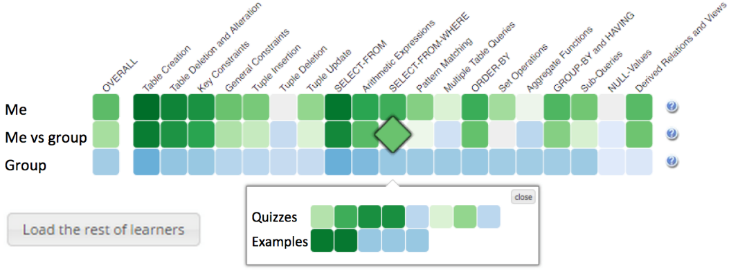
\includegraphics[width=1.0\textwidth]
    {image/brusilovsky_fig1a.png}
    \caption{Model Konseptual Antarmuka Pembelajaran
    Sosial (OSSM) (diadaptasi dari \textcite{Brusilovsky2016})}
    \label{fig:model-konseptual-sosial}
\end{figure}

Dalam implementasinya pada sistem MasteryGrids,
OSSM melengkapi aspek kognitif dengan aspek sosial melalui antarmuka yang
menampilkan visualisasi perbandingan kinerja "\textit{Me vs group}" (Saya vs grup)
dan baris "\textit{Group}" (Grup). Meskipun studi mereka menemukan bahwa fitur
eksplorasi sosial ini dapat meningkatkan pembelajaran, terutama bagi siswa
dengan pengetahuan awal rendah, pendekatan ini pada utamanya bersifat visualisasi
sosial. \textcite{Brusilovsky2016} menempatkan aspek sosial sebagai
\textit{output} untuk memotivasi siswa, namun tidak merinci bagaimana data
perbandingan sosial ini diintegrasikan kembali sebagai \textit{input} ke
dalam algoritma asesmen inti (seperti \textit{Elo rating} atau BKT) untuk
mengubah perhitungan kemahiran individu secara dinamis atau merekomendasikan
intervensi kolaboratif.

\section{Upaya Penyelesaian Masalah \textit{Over-Personalization} yang Ada Saat Ini}
\label{sec:upaya_penyelesaian}

Masalah \textit{overpersonalization} telah menjadi perhatian utama dalam penelitian sistem rekomendasi modern karena dampaknya dalam menciptakan \textit{filter bubbles} dan \textit{echo chambers}. Untuk mengatasi isolasi pengguna ini tanpa mengorbankan relevansi secara signifikan, peneliti telah mengembangkan berbagai pendekatan teknis yang inovatif. Tiga pendekatan yang paling menonjol dan relevan melibatkan penggunaan rekomendasi berbasis kelompok (\textit{Group Recommender Systems}), pemberian kendali kepada pengguna (\textit{User Controllable Systems}), dan pemodelan komunitas secara implisit (\textit{Implicit Community Modeling}).

\subsection{Sistem Rekomendasi yang Dapat Dikontrol Pengguna (\textit{User Controllable Recommender Systems})}
\label{subsec:ucrs}

Pendekatan pertama adalah pendekatan yang dikenal sebagai \textbf{\textit{User Controllable
Recommender System}} (UCRS), pendekatan ini menerapkan sistem yang memungkinkan
pengguna memiliki hak untuk
memutuskan apakah ingin menghindari \textit{filter bubble} sehingga bisa
melakukan pemilihan
"\textit{bubble}" mana yang akan menghindari. Secara fungsional,
\textcite{Wang2022} menjelaskan bahwa UCRS dapat memperingatkan pengguna jika
mereka terjebak dalam \textit{filter bubble}, mendukung empat jenis perintah
kontrol bagi pengguna untuk memitigasi \textit{bubble} pada tingkat granularitas (tingkat kedetailan)
yang
berbeda (\textit{fine-grained} dan \textit{coarse-grained}), serta merespons
kontrol tersebut dan menyesuaikan rekomendasi secara langsung (\textit{on the
fly}). Sistem ini menyediakan perintah kontrol terkait fitur pengguna atau fitur
item, seperti perintah \textit{fine-grained} untuk meningkatkan item yang disukai oleh
kelompok pengguna lain atau item dalam kategori target tertentu \autocite{Wang2022}.

\begin{figure}[!ht] 
    \centering
    \captionsetup{justification=centering}
    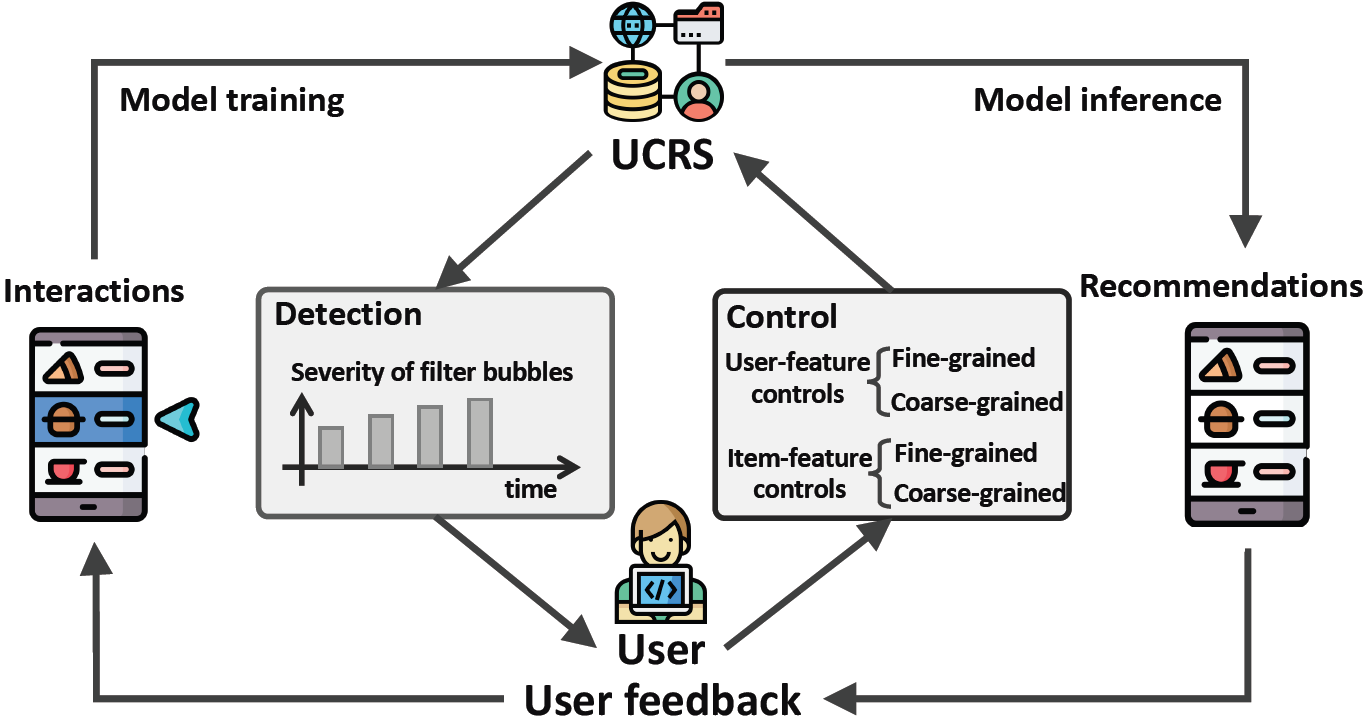
\includegraphics[width=1.0\textwidth]
    {image/UCRS_model.png}
    \caption{Model Konseptual Sistem Rekomendasi
    yang Dapat Dikontrol Pengguna (UCRS)
    (diadaptasi dari \textcite{Wang2022})}
    \label{fig:model-konseptual-UCRS}
\end{figure}

Tantangan teknis utama dalam merespons kontrol pengguna adalah memblokir efek dari
representasi pengguna yang sudah kedaluwarsa (\textit{out-of-date}), yang
mengandung informasi historis yang tidak konsisten dengan perintah kontrol.
Untuk mengatasi hal ini, dikembangkan kerangka kerja \textbf{\textit{User
Controllable Inference}} (UCI) yang ditingkatkan dengan kausalitas, yang
memeriksa prosedur pembuatan rekomendasi dari pandangan kausal dan
memanfaatkan inferensi kontrafaktual (\textit{counterfactual inference})
untuk memitigasi efek dari representasi pengguna yang kedaluwarsa tersebut
\autocite{Wang2022}. Secara khusus, UCI membayangkan dunia kontrafaktual yang di dalamnya
representasi pengguna yang kedaluwarsa dibuang, dan mengestimasi efeknya sebagai
perbedaan antara dunia faktual dan kontrafaktual, lalu mengurangi efek tersebut 
dalam prediksi akhir.

\subsection{Pendekatan Berbasis Kelompok (\textit{Group Recommender Systems})}
\label{subsec:grs}

Pendekatan kedua menggunakan \textbf{\textit{Group Recommender Systems}} (GRS)
untuk memitigasi masalah \textit{filter bubble} dan \textit{echo chamber} dengan
fokus pada kelompok pengguna yang besar. \textcite{Dokoupil2022} mengusulkan
aplikasi baru GRS yang melibatkan konstruksi kelompok pengguna skala besar dan
berfokus pada keadilan jangka panjang (\textit{long-term fairness}) dari
kelompok-kelompok ini, yang berbeda dengan penelitian yang sudah ada sebelumnya yang berkonsentrasi
pada kelompok kecil yang bersifat sementara. GRS perlu mengatasi heterogenitas
preferensi anggota kelompok dan menghasilkan rekomendasi dengan utilitas
keseluruhan yang tinggi sambil tetap mempertimbangkan rasa keadilan di antara
anggota kelompok \autocite{Dokoupil2022}.

Secara spesifik untuk skenario pengguna tunggal, pendekatan ini mengusulkan
pembangunan \textit{"virtual groups"} atau kelompok virtual yang kemudian
diteruskan ke GRS untuk mendapatkan rekomendasi akhir bagi pengguna tersebut.
Hipotesis awalnya adalah bahwa anggota kelompok virtual seharusnya fokus pada
topik yang serupa, tetapi dapat memiliki sikap yang beragam terhadap topik
tersebut \autocite{Dokoupil2022}. Dengan menerapkan GRS pada kelompok yang
seimbang (mungkin besar) alih-alih rekomendasi individu, pendekatan ini
bertujuan untuk meningkatkan pluralitas opini atau mengurangi polarisasi,
sehingga membantu memecahkan masalah \textit{filter bubble}. Meskipun demikian,
perlu dicatat bahwa pekerjaan ini masih merupakan rencana penelitian untuk
aplikasi baru GRS sehingga penulis masih baru merencanakan investigasi terhadap
efek ukuran kelompok pada kinerja GRS serta evaluasi menggunakan grup yang
dihasilkan secara sintetis maupun data publik \autocite{Dokoupil2022}.

\subsection{Pemodelan Komunitas Implisit untuk Memecahkan \textit{Echo Chamber}}
\label{subsec:frediech}

Pendekatan ketiga adalah \textbf{FRediECH} (\textit{A Friend RecommenDer for
breaking Echo CHambers}), sebuah pendekatan rekomendasi teman yang sadar akan
\textit{echo chamber} dan bertujuan merekomendasikan teman yang relevan dan
beragam dari luar jangkauan pengaruh \textit{echo chamber} pengguna. Pendekatan
ini didasarkan pada pembelajaran representasi pengguna dan \textit{echo chamber}
secara dinamis berdasarkan konten yang dibagikan dan interaksi komunitas pengguna,
alih-alih bergantung pada penemuan komunitas secara eksplisit yang mungkin
kompleks secara komputasi \autocite{Tommasel2021}. Masalah rekomendasi
diformulasikan untuk mempelajari fungsi yang mengestimasi kekuatan interaksi
potensial antar pengguna berdasarkan interaksi masa lalu dan konten yang
dibagikan, pada formulasi ini kekuatan interaksi potensial yang
lebih tinggi menunjukkan keseimbangan yang
lebih baik antara relevansi pengguna dan jaraknya dari \textit{echo chamber}
pengguna lain.

\begin{figure}[!ht] 
    \centering
    \captionsetup{justification=centering}
    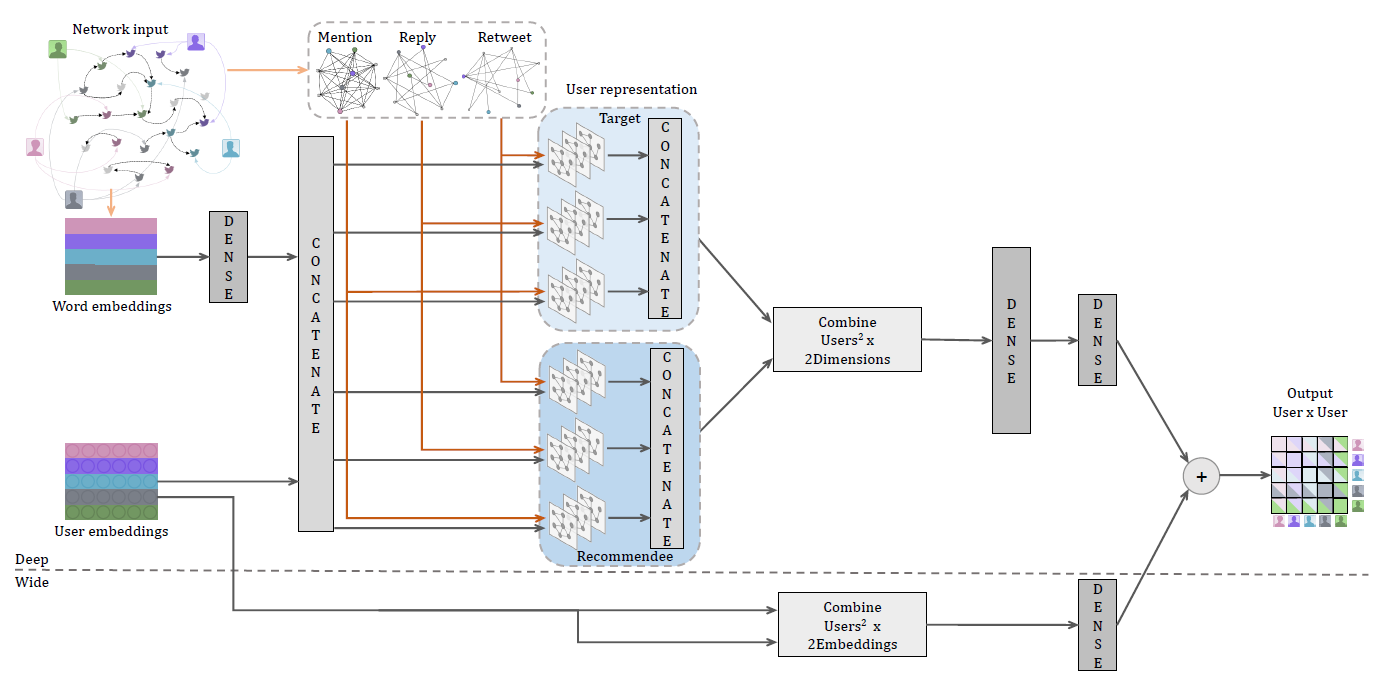
\includegraphics[width=1.0\textwidth]
    {image/FRediECH_architecture.png}
    \caption{Diagram Arsitektur FRediECH
    (diadaptasi dari \textcite{Tommasel2021})}
    \label{fig:arsitektur-FRediECH}
\end{figure}

Pada gambar \ref{fig:arsitektur-FRediECH} terlihat arsitektur FRediECH
yang terinspirasi oleh \textbf{\textit{Graph Convolutional
Network}} (GCN) dan arsitektur \textbf{\textit{Deep \& Wide}}, yang
menggabungkan kesadaran \textit{echo chamber} dan representasi pengguna untuk
menyeimbangkan relevansi, keragaman, dan kebaruan rekomendasi.
\textcite{Tommasel2021} menggunakan GCN paralel untuk mempelajari kontribusi 
spesifik dari jenis interaksi tertentu (seperti \textit{reply}, \textit{mention},
atau \textit{retweet}) terhadap set lengkap hubungan pengguna, kemudian
menggabungkan outputnya untuk menghasilkan representasi pengguna perantara.
Fungsi kerugian (\textit{loss function}) didefinisikan berdasarkan jarak antara
pengguna dan jumlah interaksi, yang bertujuan untuk memberikan bobot pada
interaksi sedemikian rupa sehingga interaksi antara pengguna yang berasal dari
\textit{echo chamber} yang berbeda membawa bobot yang lebih tinggi daripada
interaksi dalam \textit{echo chamber} yang sama sehingga mempromosikan keragaman
rekomendasi dengan mempelajari struktur komunitas secara implisit
\autocite{Tommasel2021}.

\subsection{Mitigasi Dampak \textit{Echo Chamber} Melalui \textit{Constraint-Based Re-ranking}}
\label{ssec:debiasio_reranking}

Salah satu pendekatan algoritmik terbaru yang secara spesifik menangani dampak rekomendasi terhadap perilaku pengguna adalah kerangka kerja yang diusulkan oleh \textcite{DeBiasio2023}. Penelitian ini membedakan dirinya dari pendekatan diversifikasi umum dengan memfokuskan pada perlindungan kelompok pengguna "sensitif" (\textit{sensitive users}) dari paparan berlebih terhadap konten "berpengaruh" (\textit{influential items}) yang dapat memperburuk kondisi perilaku mereka, seperti polarisasi ekstrem atau isolasi sosial.

% \subsubsection{Konsep Pengguna Sensitif dan Item Berpengaruh}
Dalam model \textcite{DeBiasio2023}, masalah \textit{echo chamber} tidak dipandang seragam untuk semua pengguna, melainkan diklasifikasikan berdasarkan kerentanan:
\begin{enumerate}
    \item \textbf{Pengguna Sensitif (\textit{Sensitive Users}):} Kelompok pengguna yang perilakunya rentan dipengaruhi secara negatif oleh pola konsumsi konten yang homogen atau bias.
    \item \textbf{Item Berpengaruh (\textit{Influential Items}):} Kategori konten yang memiliki dampak signifikan terhadap perilaku pengguna sensitif. Item ini dibagi menjadi dua:
    \begin{enumerate}
        \item \textit{Controversial Items}: Item yang jika dikonsumsi berlebihan dapat memperburuk isolasi atau perilaku negatif.
        \item \textit{Favorable Items}: Item yang dapat memberikan dampak positif atau memecah isolasi (\textit{bubble}) jika direkomendasikan dengan proporsi yang cukup.
    \end{enumerate}
\end{enumerate}

Pendekatan ini sangat relevan untuk konteks pembelajaran adaptif karena "pengguna sensitif" dapat dipetakan sebagai siswa yang terisolasi secara akademik, dan "favorable items" sebagai interaksi dengan rekan yang memiliki kompetensi berbeda (heterogen).

% \subsubsection{Algoritma \textit{Re-ranking} Berbasis Batasan}
Untuk memitigasi dampak negatif rekomendasi pada pengguna sensitif tanpa memerlukan pelatihan model ulang, \textcite{DeBiasio2023} mengusulkan algoritma \textit{greedy re-ranking}. Algoritma ini bekerja pada tahap pasca-pemrosesan dengan menyusun ulang daftar skor prediksi awal ($\hat{r}_u$) agar memenuhi batasan proporsi item tertentu.

Pada kode \ref{alg:reranking_debiasio_original} diperlihatkan pseudocode dari algoritma \textit{re-ranking} tersebut sebagaimana didefinisikan dalam penelitian aslinya.

\begin{minipage}{\textwidth} 
\begin{lstlisting}[frame=lines, captionpos=t, caption={Algoritma Re-ranking}, label={alg:reranking_debiasio_original}]
ALGORITHM Re-ranking
    INPUT:
        u      : User identifier
        S      : Set of sensitive users
        r_hat  : Scores predicted by backbone model for user u
        alpha  : Minimum percentage of favorable items allowed
        beta   : Maximum percentage of controversial items allowed
        k      : Number of items to be recommended
    OUTPUT:
        Y_star : Top-k items to recommend to user u
    BEGIN
        IF u NOT IN S THEN
            RETURN Argsort(r_hat, order='descending')[0:k]
        
        ELSE
            Y_star <- EmptySet
            SortedItems <- Sort(r_hat, order='descending')
            
            FOR EACH item j IN SortedItems DO
                IF Size(Y_star) < k THEN
                    
                    CondAlpha <- ((f_j + Sum(f_i for i in Y_star)) / k) >= alpha
                    
                    CondBeta  <- ((c_j + Sum(c_i for i in Y_star)) / k) <= beta
                    
                    IF CondAlpha AND CondBeta THEN
                        Add j to Y_star
                    END IF
                ELSE
                    BREAK
                END IF
            END FOR
            
            RETURN Y_star
        END IF
    END
END ALGORITHM
\end{lstlisting}
\end{minipage}

Secara matematis, algoritma memastikan bahwa probabilitas terpilihnya
suatu item $y_i$ dalam rekomendasi untuk pengguna sensitif ($s_u=1$) memenuhi
pertidaksamaan berikut,

\begin{align}
    \mathbb{P}(y_i=1 \mid s_u=1, f_i=1) &\geq \alpha \label{eq:constraint_favorable} \\
    \mathbb{P}(y_i=1 \mid s_u=1, c_i=1) &\leq \beta \label{eq:constraint_controversial}
\end{align}

dengan:
\begin{itemize}
    \item Persamaan \eqref{eq:constraint_favorable} menetapkan bahwa proporsi
    item \textit{favorable} (yang memecah isolasi) harus lebih besar atau sama
    dengan ambang batas $\alpha$.
    \item Persamaan \eqref{eq:constraint_controversial} menetapkan bahwa proporsi
    item \textit{controversial} (yang memperburuk isolasi) harus lebih kecil
    atau sama dengan ambang batas $\beta$.
\end{itemize}

% \subsubsection{Mekanisme Kerja Algoritma}
Algoritma \textit{re-ranking} ini bekerja dengan menyusun ulang daftar
rekomendasi $\mathcal{Y}_{u,k}$ secara iteratif. Pada setiap langkah penambahan
item ke dalam daftar rekomendasi final, algoritma memeriksa apakah penambahan
item tersebut akan melanggar batasan $\alpha$ atau $\beta$.
\begin{itemize}
    \item Jika daftar rekomendasi saat ini kekurangan item \textit{favorable}
    (di bawah ambang $\alpha$), algoritma akan secara paksa mengambil item
    \textit{favorable} dari daftar cadangan, meskipun skor relevansinya sedikit
    lebih rendah, untuk menggantikan item non-favorable.
    \item Mekanisme ini menjamin terjadinya "eksposur paksa" (\textit{forced
    exposure}) terhadap konten yang beragam, yang merupakan syarat utama untuk
    memecahkan \textit{filter bubble} secara efektif \autocite{DeBiasio2023}.
\end{itemize}

Keunggulan utama pendekatan ini adalah sifatnya yang \textit{model-agnostic} dan
efisien secara komputasi karena menggunakan pendekatan \textit{greedy} pada
tahap \textit{post-processing}, sebagaimana dijelaskan secara teknis oleh
\textcite{DeBiasio2023}. Hal ini membuatnya lebih layak diimplementasikan pada
kondisi data terbatas (\textit{cold-start}) dibandingkan metode berbasis
\textit{Deep Learning} yang membutuhkan pelatihan ekstensif.

\subsection{Evaluasi Efektivitas Pembelajaran dengan \textit{Normalized Learning Gain}}

Dalam ranah penelitian pendidikan fisika dan teknologi pembelajaran, pengukuran
efektivitas intervensi instruksional sering kali menghadapi tantangan bias yang
disebabkan oleh perbedaan tingkat pengetahuan awal siswa. Untuk mengatasi hal
ini, Richard Hake memperkenalkan konsep \textit{average normalized gain} ($g$)
sebagai metrik standar. Secara teoretis, \textit{normalized gain} didefinisikan
sebagai rasio antara peningkatan skor aktual yang dicapai (\textit{actual gain})
terhadap peningkatan skor maksimum yang mungkin dicapai (\textit{maximum possible
gain}). Penggunaan metrik ini bertujuan untuk memisahkan efek pembelajaran dari
pengaruh skor \textit{pre-test} sehingga memungkinkan perbandingan yang objektif
antara populasi siswa yang memiliki latar belakang kemampuan yang heterogen
\autocite{Nissen2018}.

Secara matematis, perhitungan \textit{normalized gain} untuk rata-rata kelas
atau individu dinyatakan dalam persamaan berikut, dengan asumsi skor dinyatakan
dalam persentase:

\begin{align}
    g &= \frac{\%\text{post} - \%\text{pre}}{100 - \%\text{pre}} \label{eq:normalized_gain_formula}
\end{align}

dengan $\%\text{pre}$ merepresentasikan persentase skor pada tes awal sebelum
instruksi diberikan, dan $\%\text{post}$ adalah persentase skor pada tes akhir.
\textcite{Coletta2020} menegaskan bahwa metrik ini memiliki keunggulan teoretis
dibandingkan perhitungan selisih skor mentah atau \textit{effect size} standar
(seperti Cohen's $d$), terutama dalam menangani distribusi data yang mengalami
\textit{floor effect} atau \textit{ceiling effect} ekstrem, sebuah efek yang
mengakibatkan siswa dengan
skor awal tinggi memiliki ruang peningkatan yang lebih sempit dibandingkan siswa
dengan skor rendah.

Sebagai standar interpretasi efektivitas yang berlaku umum dalam literatur, Hake
menetapkan kriteria ambang batas untuk mengkategorikan tingkat keberhasilan
pembelajaran. Nilai $g$ diklasifikasikan ke dalam tiga kategori: (1)
\textbf{Rendah} (\textit{Low-g}) jika $g < 0.3$; (2) \textbf{Sedang}
(\textit{Medium-g}) jika $0.3 \leq g < 0.7$; dan (3) \textbf{Tinggi}
(\textit{High-g}) jika $g \geq 0.7$. Klasifikasi ini menyediakan kerangka kerja
komparatif yang konsisten bagi para peneliti untuk mengevaluasi apakah sebuah
metode pedagogis mampu menghasilkan peningkatan pemahaman konsep yang substansial
terlepas dari kesulitan materi yang diajarkan \autocite{Coletta2020}.